O \textit{boxplot}, também conhecido como diagrama de extremos e quartis, é uma ferramenta gráfica recorrente em Estatística, que permite visualizar a distribuição de um conjunto unidimensional de dados\cite{casella2002statistical} \cite{ross2014introduction}. Esta ferramenta, proposta por John Tukey, em 1970, permite compreender o comportamento da distribuição dos dados, da sua dispersão e simetria. A informação obtida pelo \textit{boxplot} resulta dos seguintes componentes: 


\begin{my_itemize}
	
	\item \textbf{Quartis}: Os quartis são os valores que dividem um conjunto de dados ordenados em quatro partes iguais, contendo cada uma 25\% dos dados. Para o respetivo cálculo, é necessário organizar os dados por ordem crescente. Ao primeiro quartil ($Q_1$), também conhecido como quartil inferior, corresponde o valor abaixo do qual se encontram 25\% dos dados ordenados. O segundo quartil ($Q_2$), ou mediana, é o valor abaixo do qual se encontram 50\% dos dados ordenados. O terceiro quartil ($Q_3$), conhecido como quartil superior, é o valor abaixo do qual se encontram 75\% dos dados ordenados.
	
	\item \textbf{Caixa}: Representa o intervalo interquartil (IQR). Neste intervalo estão contidos  todos os dados cujo valor é superior ao primeiro quartil ($Q_1$) e inferior ao terceiro quartil ($Q_3$), contemplando 50\% dos dados. A caixa permite, assim, verificar a dispersão dos dados. Uma caixa maior corresponde a uma maior variabilidade dos dados, ao passo que uma caixa menor indica uma maior concentração. 
	
	\item \textbf{Mediana}: É a linha que se encontra dentro da caixa e é denominada de mediana ($Q_2$). Esta linha divide o conjunto de dados em duas metades iguais. A partir da localização da mediana dentro da caixa pode-se observar, ou não, a presença de uma assimetria na distribuição dos dados. Se a linha se encontrar no meio, ou muito perto do meio da caixa, significa que a distribuição dos dados tende a ser simétrica. Por outro lado, se esta estiver deslocada para um dos lados significa que o conjunto de dados é assimétrico. 
	
	\item \textbf{Extremidades (Whiskers)}: São as linhas que se estendem desde os primeiro e terceiro quartis até aos valores mais extremos do conjunto de dados, que não sejam considerados \textit{outliers}. Existem diferentes formas de definir estas extremidadas\cite{spe}  mas, geralmente, são definidas através do seguinte intervalo: 
	
		\begin{equation}
			\text{I} = [Q_1 - 1.5 \hspace{1px} \text{IQR} \hspace{2px} , \hspace{2px} Q_3 + 1.5 \hspace{1px} \text{IQR}]
			\label{eq:out}
		\end{equation} 
	
	\item \textbf{Outliers}: São todos os pontos que não são abrangidos pelas extremidades. São valores diferentes dos demais e são representados por pontos individuais. A existência de um elevado número de outliers pode indicar a presença de distribuições com caudas longas e a presença de valores extremos. 
	Contudo, existem autores que estabelecem uma distinção entre \textit{ouliers} moderados (Equação \ref{eq:outmod}) e \textit{outliers} severos (Equação \ref{eq:outsev})\cite{spe}.
	
	
	\begin{equation}
		\text{I}_{mod} = [Q_1 - 3 \cdot\text{IQR} , \hspace{2px} Q_1 - 1.5 \cdot\text{IQR}] \cup 
		[Q_3 + 1.5 \cdot\text{IQR} , \hspace{2px} Q_3 + 3 \cdot\text{IQR}]
		\label{eq:outmod}
	\end{equation}
	
	\begin{equation}
		\text{I}_{sev} = ] -\infty, Q_1 - 3 \cdot\text{IQR}[ \cup ]Q_3 + 3 \cdot\text{IQR},+\infty[
		\label{eq:outsev}
	\end{equation}
	
	Na Figura \ref{fig:outliers} pode observar-se uma representação destes intervalos.
	
\end{my_itemize}

\begin{figure}[H]
	\centering
	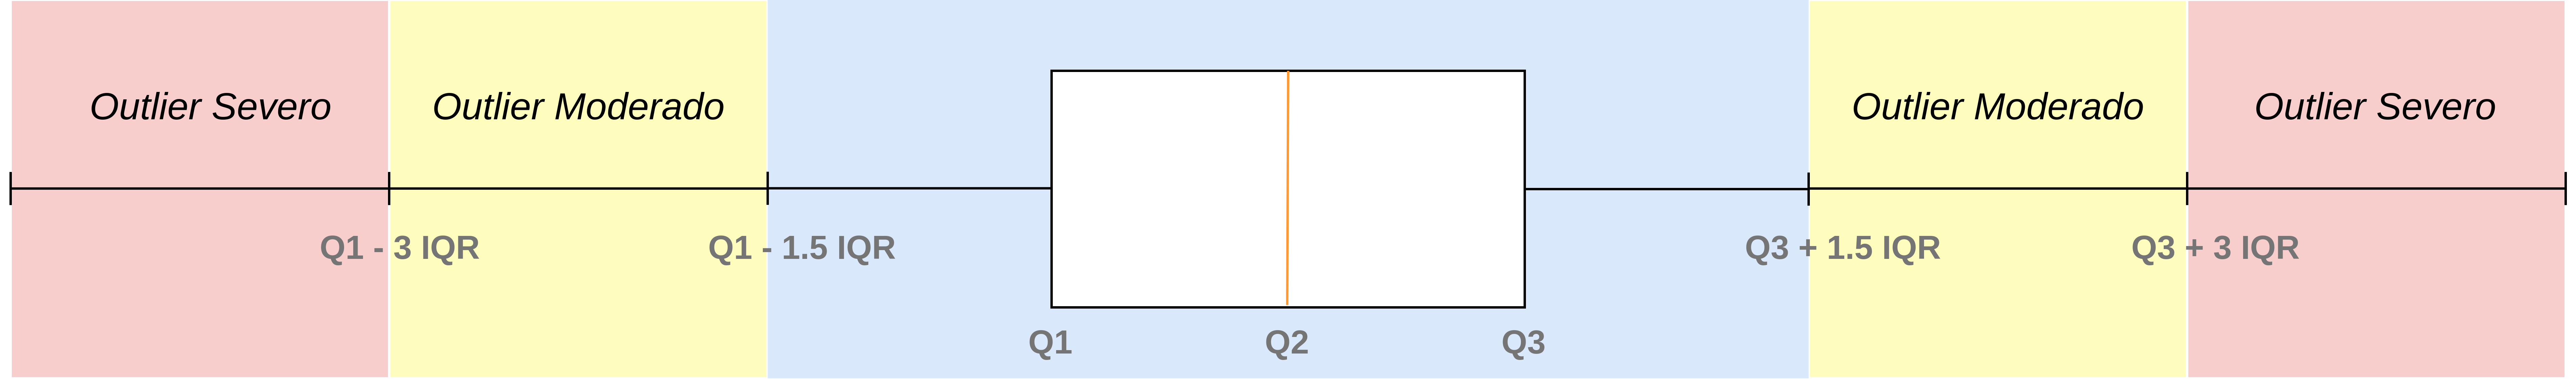
\includegraphics[width=\textwidth]{imagens/boxplot.png}
	\caption{\textit{Outliers} moderados e severos num diagrama de caixa e bigodes.}
	\label{fig:outliers}
\end{figure}

Os \textit{boxplots} permitem obter uma visão da distribuição dos dados, identificando rapidamente \textit{outliers} e assimetrias para uma amostra com um número de observações estatisticamente significativo. Contudo, esta ferramenta não apresenta a informação dos dados de uma forma completa e, por isso, é frequentemente acompanhado de um histograma.

\begin{figure}[H]
	\centering
	\includegraphics[width=\textwidth]{imagens/stats/hist2.png}
	\caption{Histograma e \textit{boxplot} para diferentes distribuições.}
	\label{fig:histos}
\end{figure}

Na Figura \ref{fig:histos} podem observar-se três cenários distintos. Cada uma das amostras é composta por 1000 pontos, gerados a partir das bibliotecas Numpy e Scipy do Python \cite{python}. A primeira amostra foi gerada a partir de uma distribuição normal com valor médio 0 e uma variância de 0.5, a segunda a partir de uma distribuição normal com valor médio 0 e variância 1, ambas geradas pelo módulo \textit{numpy.random.norm}, e a terceira a partir de uma distribuição normal assimétrica, usando o módulo \textit{scipy.stats.skewnorm}. A partir da observação dos dois primeiros gráficos verifica-se que a distância interquartil do primeiro é inferior à do segundo, consequência de uma menor variância dos dados. No terceiro gráfico observa-se uma distribuição assimétrica à esquerda. A partir do \textit{boxplot} correspondente, verifica-se que os \textit{whiskers} não têm o mesmo tamanho e a mediana situa-se mais próxima do primeiro quartil do que do terceiro, em resultado de uma maior concentração dos dados à esquerda. 


\section{Outliers em distribuições assimétricas}

Os \textit{outliers} representam uma componente fundamental na interpretação e análise de dados. A sua origem pode dever-se a fatores naturais, ou seja, existe efetivamente uma possibilidade, ainda que remota, de se observar este evento. Outras vezes, deve-se a erros de medição, de digitação e outros erros de origem humana. Uma única observação não concordante com as demais pode modificar a conclusão de um estudo e, como tal, é motivo de cautela para estatísticos e analistas de dados. A definição de \textit{outlier} não é consensual e, nesse sentido, os modelos e métodos de selecção e detecção de valores aberrantes numa amostra são fundamentais. Uma das várias maneiras de descrever um \textit{outlier} passa por considerá-los como pontos que são discordantes dos restantes, tornando-se, assim, pontos \textit{suspeitos}\cite{spe}. Desta forma, colocam-se as seguintes questões: o que torna uma observação suspeita e a partir de que \textit{distância} é que um ponto de uma amostra se torna suspeito? 


Como referido anteriormente, ao representar-se um conjunto de pontos através de um \textit{boxplot}, um \textit{outlier} é, geralmente, qualquer ponto que não pertença ao intervalo $\left[Q_1 - 1.5\text{IQR}, Q_3 + 1.5 \text{IQR} \right]$. Este intervalo é definido a partir de uma amostra de pontos que segue uma distribuição normal. 
Convencionou-se que, em média, de um conjunto de pontos que segue uma distribuição normal, apenas 0.7\% devem corresponder a outliers, estando igualmente repartidos para os dois lados da distribuição \cite{hoaglin1983understanding}. De modo a ilustrar a afirmação anterior, foi realizada uma simulação em Python, cujo código se encontra presente na secção \ref{lst:normalcode}, a qual comprovou que a percentagem média de \textit{outliers}, para ambos os lados da distribuição é 0.35\%. O resultado encontra-se na Figura \ref{fig:normalouts}. 

Desta forma, nas amostras que sigam distribuições diferentes da distribuição normal, nem todos os pontos não pertencentes ao intervalo definido pela Equação \ref{eq:out} são necessáriamente outliers reais \cite{hoaglin1983understanding} e, como tal, em última análise, devem ser considerados como \textit{potenciais} \textit{outliers}. Este facto revela-se de especial importância quando são consideradas distribuições com caudas longas, onde existem muitas observações que excedem os limites superior e inferior das extremidades, ou em distribuições assimétricas. Por exemplo, em distribuições assimétricas à direira existe um reduzido número de pontos que ultrapassa o limite inferior da extremidade. Por outro lado, existe um número significativo de pontos que ultrapassa o limite superior da extremidade. Na Figura \ref{fig:histos} evidencia-se este facto através da observação do \textit{boxplot} do gráfico da direita, onde se constata que o número de outliers é bastante superior relativamente aos outros dois cenários. Contudo, muitos destes outliers são mal classificados devido à forma como as extremidades são definidas. 

Por forma a solucionar a questão da assimetria de uma distribuição, foi proposto um ajuste relativamente à definição das extremidades do boxplot convencional (Hubert e Vandervieren, 2007) \cite{hoaglin1983understanding}. Este ajuste resulta numa generalização do boxplot que pode ser aplicado a todas as distribuições, tem em conta a sua simetria e evita a má classificação de \textit{outliers}. Para realizar este ajuste é preciso ter em conta a medida de simetria de uma distribuição, obtida pela constante de Medcouple \cite{mc}. 

Considere-se uma amostra unidimensional ${x_1, \dots, x_n}$ gerada a partir de uma distribuição F. A constante de Medcouple é definida da seguinte forma:


\begin{equation}
	\text{MC} = \operatorname*{med}_{\substack{x_i \leq Q_2 \leq x_j}} h(x_i, x_j) = \operatorname*{med}_{\substack{x_i \leq Q_2 \leq x_j}} \frac{(x_j - Q_2) - (Q_2 - x_i)}{x_j - x_i}
\end{equation}

Esta fórmula é definida para qualquer $x_i \neq x_j$ e toma sempre valores pertencentes ao intervalo $[-1,1]$. Para distribuições assimétricas à direita, assimétricas à esquerda e simétricas, o valor da constante de Medcouple toma, respetivamente, valores positivo, negativo e, aproximadamente, nulo. A Figura \ref{fig:histmc} ilustra o enunciado anteriormente.

\begin{figure}[H]
	\centering
	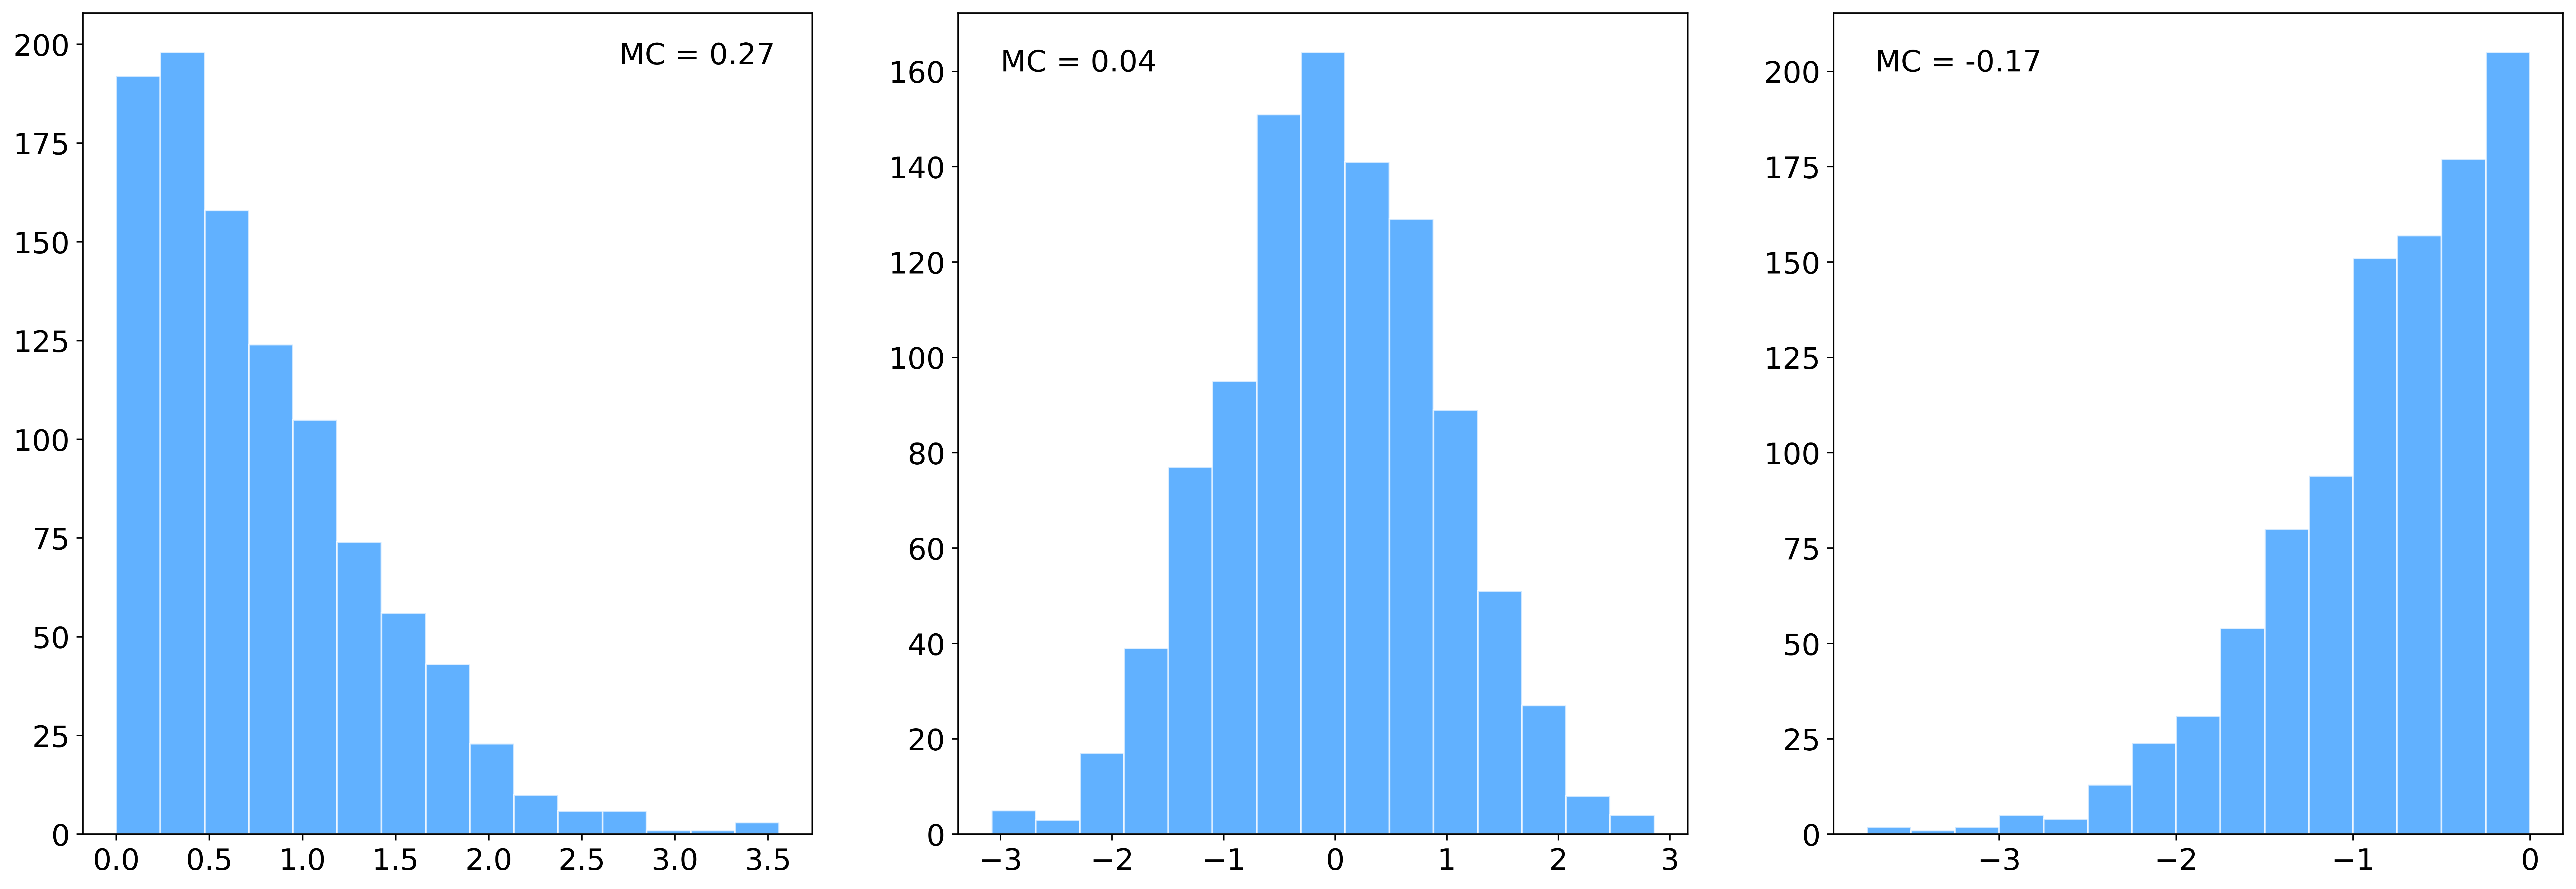
\includegraphics[width=\textwidth]{imagens/stats/histos_mc.png}
	\caption{Valores da constante de Medcouple para diferentes distribuições.}
	\label{fig:histmc}
\end{figure}


Com o objetivo de ajustar o \textit{boxplot} à simetria do conjunto de dados, foi proposto que o intervalo apresentado na Equação \ref{eq:out} sofresse as seguintes modificações, de forma a contemplar a constante de Medcouple na definição dos \textit{whiskers}:


\begin{equation}
	\text{I} = [Q_1 - h_l(\text{MC}) \hspace{1px} \text{IQR} \hspace{2px} , \hspace{2px} Q_3 + h_u(\text{MC}) \hspace{1px} \text{IQR}]
	\label{eq:outalt}
\end{equation}


Aqui, $h_l(\text{MC})$ e $h_u(\text{MC})$ são funções a modelar. De forma a garantir que se obtém o \textit{boxplot} convencional para distribuições simétricas é necessário garantir que $h_l(0) = h_u(0) = 1.5$. Ou seja, quando uma distribuição é simétrica, a constante de Medcouple é nula e, por sua vez, o intervalo definido na Equação \ref{eq:outalt} passa a ser igual ao da Equação \ref{eq:out}. Foram considerados três modelos distintos ao longo deste estudo:

\begin{center}
	\begin{tabular}{>{\centering\arraybackslash}m{4cm} >{\centering\arraybackslash}m{5cm} >{\centering\arraybackslash}m{5cm}}
		\textbf{Modelo Linear} & \textbf{Modelo Quadrático} & \textbf{Modelo Exponencial} \\
		\(\begin{aligned} 
			h_l(\text{MC}) &= 1.5 + a\text{MC} \\ 
			h_u(\text{MC}) &= 1.5 + b\text{MC} 
		\end{aligned}\) & 
		\(\begin{aligned} 
			h_l(\text{MC}) &= 1.5 + a_1\text{MC} + a_2\text{MC}^2\\ 
			h_u(\text{MC}) &= 1.5 + b_1\text{MC} + b_2\text{MC}^2
		\end{aligned}\) & 
		\(\begin{aligned} 
			h_l(\text{MC}) &= 1.5 e^{a\text{MC}} \\ 
			h_u(\text{MC}) &= 1.5 e^{b\text{MC}} 
		\end{aligned}\) \\
	\end{tabular}
\end{center}

com $a,a_1,a_2,b,b_1,b_2 \in \mathbb{R}$. Para derivar estas constantes foram utilizadas diversas distribuições\footnote{Foram utilizadas distribuições $\Gamma$, $\chi^2$, Pareto, entre outras}, onde se tentaram definir extremidades de modo que, a percentagem de outliers fosse aproximadamente 0.7\%, à semelhança do \textit{boxplot} convencional, e cujo valor da constante de Medcouple não fosse superior a 0.6. Desta forma, não foram consideradas distribuições muito assimétricas.

O modelo que apresentou um melhor desempenho na determinação de extremidades foi o exponencial, com valores estimados de $a = -4$ e $b = 3$. Assim, Hubert e Vandervieren (2007), sugerem que sejam utilizados os seguintes intervalos, consoante a assimetria da distribuição, na construção dos boxplots: 

\begin{align}
	\text{MC} \geq 0: & \quad [Q_1 -  1.5 e^{-4\text{MC}} \hspace{1px} \text{IQR} \hspace{2px} , \hspace{2px} Q_3 + 1.5 e^{3\text{MC}} \hspace{1px} \text{IQR}] 	\label{eq:medatual1} \\ \vspace{3px}
	\text{MC} < 0: & \quad [Q_1 -  1.5 e^{-3\text{MC}} \hspace{1px} \text{IQR} \hspace{2px} , \hspace{2px} Q_3 + 1.5 e^{4\text{MC}} \hspace{1px} \text{IQR}]
	\label{eq:medatual}
\end{align}

É de salientar que este boxplot ajustado não tem em conta distribuições com caudas longas, mas apenas distribuições assimétricas.
















































